\documentclass[10pt, twocolumn, letterpaper]{article}

%%%%%%%%% PAPER TYPE  - PLEASE UPDATE FOR FINAL VERSION
\usepackage{cvpr}
\usepackage{cite}
              % To produce the CAMERA-READY version
% \usepackage[review]{cvpr}      % To produce the REVIEW version
% \usepackage[pagenumbers]{cvpr} % To force page numbers, e.g. for an arXiv version

% Import additional packages in the preamble file, before hyperref
\usepackage[dvipsnames]{xcolor}
\newcommand{\red}[1]{{\color{red}#1}}
\newcommand{\todo}[1]{{\color{red}#1}}
\newcommand{\TODO}[1]{\textbf{\color{red}[TODO:#1]}}


% It is strongly recommended to use hyperref, especially for the review version.
% hyperref with option pagebackref eases the reviewers' job.
% Please disable hyperref *only* if you encounter grave issues, 
% e.g. with the file validation for the camera-ready version.
%
% If you comment hyperref and then uncomment it, you should delete *.aux before re-running LaTeX.
% (Or just hit 'q' on the first LaTeX run, let it finish, and you should be clear).
\definecolor{cvprblue}{rgb}{0.21, 0.49, 0.74}
\usepackage[pagebackref,breaklinks,colorlinks,citecolor=cvprblue]{hyperref}
% \bibliographystyle{ieee}
% \bibliography{references}


%%%%%%%%% PAPER ID  - PLEASE UPDATE
\def\paperID{*****} % *** Enter the Paper ID here
\def\confName{CVPR}
\def\confYear{2024}

% It is strongly recommended to use hyperref, especially for the review version.
% hyperref with option pagebackref eases the reviewers' job.
% Please disable hyperref *only* if you encounter grave issues, 
% e.g. with the file validation for the camera-ready version.
%
% If you comment hyperref and then uncomment it, you should delete *.aux before re-running LaTeX.
% (Or just hit 'q' on the first LaTeX run, let it finish, and you should be clear).
\definecolor{cvprblue}{rgb}{0.21, 0.49, 0.74}
\usepackage[pagebackref,breaklinks,colorlinks,citecolor=cvprblue]{hyperref}
\usepackage{graphicx}
\usepackage{listings}
\usepackage{amsmath}

%%%%%%%%% PAPER ID  - PLEASE UPDATE
\def\paperID{*****} % *** Enter the Paper ID here
\def\confName{CVPR}
\def\confYear{2024}

%%%%%%%%% TITLE - PLEASE UPDATE
\title{Tissue Segmentation during Endoscopy using Deep Learning}

%%%%%%%% AUTHORS - PLEASE UPDATE
\author{
    Pradeep Mundlik \\
    {\tt\small ai21btech11022@iith.ac.in}
    \and
    Naman Chhibhar \\
    {\tt\small ma21btech11011@iith.ac.in}
}

\begin{document}
\maketitle
\begin{abstract}
    In this project we aim to implement semantic segmentation model to help with segmentation task during Endoscopic surgery. A DeepLabV3 model with Resnet-101 as backbone and FCN head as auxillary classifier is trained. We have extracted images from POEM videos and annoted using Segment\_anything model. 
\end{abstract}
    
\section{Introduction}
\label{sec:intro}

Endoscopy is non-surgical examination of internal organs using a flexible tube with a light and camera called an Endoscope. It is an established resection technique to diagnose, treat, or monitor conditions in the digestive or respiratory tract. 
There are two major endoscopic procedures, \textbf{Endoscopic submucosal dissection (ESD)} and \textbf{Peroral Endoscopic Myotomy (POEM)}. 
%-------------------------------------------------------------------------
% \subsection{Problem Statement}
ESD and POEM are complex procedures with elevated risk of operator dependent adverse events. There are high chances of intraprocedural bleeding and perforation which lead to significant risks to patient safety and procedural success. In this project we aim to develop an Artificial Intelligence Clinical Decision Support Solution (AI-CDSS) for on-time detection of Muscle layer, Submucosal layer and Electrode; making it helpful and assisting for operator during surgery. 

% \subsection{Dual submission}

% Please refer to the author guidelines on the \confName\ \confYear\ web page for a
% discussion of the policy on dual submissions.

% \subsection{Paper length}
% Papers, excluding the references section, must be no longer than eight pages in length.
% The references section will not be included in the page count, and there is no limit on the length of the references section.
% For example, a paper of eight pages with two pages of references would have a total length of 10 pages.
% {\bf There will be no extra page charges for \confName\ \confYear.}

% Overlength papers will simply not be reviewed.
% This includes papers where the margins and formatting are deemed to have been significantly altered from those laid down by this style guide.
% Note that this \LaTeX\ guide already sets figure captions and references in a smaller font.
% The reason such papers will not be reviewed is that there is no provision for supervised revisions of manuscripts.
% The reviewing process cannot determine the suitability of the paper for presentation in eight pages if it is reviewed in eleven.

% %-------------------------------------------------------------------------
% \subsection{The ruler}
% The \LaTeX\ style defines a printed ruler which should be present in the version submitted for review.
% The ruler is provided in order that reviewers may comment on particular lines in the paper without circumlocution.
% If you are preparing a document using a non-\LaTeX\ document preparation system, please arrange for an equivalent ruler to appear on the final output pages.
% The presence or absence of the ruler should not change the appearance of any other content on the page.
% The camera-ready copy should not contain a ruler.
% (\LaTeX\ users may use options of \texttt{cvpr.sty} to switch between different versions.)

% Reviewers:
% note that the ruler measurements do not align well with lines in the paper --- this turns out to be very difficult to do well when the paper contains many figures and equations, and, when done, looks ugly.
% Just use fractional references (\eg, this line is $087.5$), although in most cases one would expect that the approximate location will be adequate.


% \subsection{Paper ID}
% Make sure that the Paper ID from the submission system is visible in the version submitted for review (replacing the ``*****'' you see in this document).
% If you are using the \LaTeX\ template, \textbf{make sure to update paper ID in the appropriate place in the tex file}.


% \subsection{Mathematics}

% Please number all of your sections and displayed equations as in these examples:
% \begin{equation}
%   E = m\cdot c^2
%   \label{eq:important}
% \end{equation}
% and
% \begin{equation}
%   v = a\cdot t.
%   \label{eq:also-important}
% \end{equation}
% It is important for readers to be able to refer to any particular equation.
% Just because you did not refer to it in the text does not mean some future reader might not need to refer to it.
% It is cumbersome to have to use circumlocutions like ``the equation second from the top of page 3 column 1''.
% (Note that the ruler will not be present in the final copy, so is not an alternative to equation numbers).
% All authors will benefit from reading Mermin's description of how to write mathematics:
% \url{http://www.pamitc.org/documents/mermin.pdf}.

% \subsection{Blind review}

% Many authors misunderstand the concept of anonymizing for blind review.
% Blind review does not mean that one must remove citations to one's own work---in fact it is often impossible to review a paper unless the previous citations are known and available.

% Blind review means that you do not use the words ``my'' or ``our'' when citing previous work.
% That is all.
% (But see below for tech reports.)

% Saying ``this builds on the work of Lucy Smith [1]'' does not say that you are Lucy Smith;
% it says that you are building on her work.
% If you are Smith and Jones, do not say ``as we show in [7]'', say ``as Smith and Jones show in [7]'' and at the end of the paper, include reference 7 as you would any other cited work.

% An example of a bad paper just asking to be rejected:
% \begin{quote}
% \begin{center}
%     An analysis of the frobnicatable foo filter.
% \end{center}

%    In this paper we present a performance analysis of our previous paper [1], and show it to be inferior to all previously known methods.
%    Why the previous paper was accepted without this analysis is beyond me.

%    [1] Removed for blind review
% \end{quote}


% An example of an acceptable paper:
% \begin{quote}
% \begin{center}
%      An analysis of the frobnicatable foo filter.
% \end{center}

%    In this paper we present a performance analysis of the  paper of Smith \etal [1], and show it to be inferior to all previously known methods.
%    Why the previous paper was accepted without this analysis is beyond me.

%    [1] Smith, L and Jones, C. ``The frobnicatable foo filter, a fundamental contribution to human knowledge''. Nature 381(12), 1-213.
% \end{quote}

% If you are making a submission to another conference at the same time, which covers similar or overlapping material, you may need to refer to that submission in order to explain the differences, just as you would if you had previously published related work.
% In such cases, include the anonymized parallel submission~\cite{Authors14} as supplemental material and cite it as
% \begin{quote}
% [1] Authors. ``The frobnicatable foo filter'', F\&G 2014 Submission ID 324, Supplied as supplemental material {\tt fg324.pdf}.
% \end{quote}

% Finally, you may feel you need to tell the reader that more details can be found elsewhere, and refer them to a technical report.
% For conference submissions, the paper must stand on its own, and not {\em require} the reviewer to go to a tech report for further details.
% Thus, you may say in the body of the paper ``further details may be found in~\cite{Authors14b}''.
% Then submit the tech report as supplemental material.
% Again, you may not assume the reviewers will read this material.

% Sometimes your paper is about a problem which you tested using a tool that is widely known to be restricted to a single institution.
% For example, let's say it's 1969, you have solved a key problem on the Apollo lander, and you believe that the 1970 audience would like to hear about your
% solution.
% The work is a development of your celebrated 1968 paper entitled ``Zero-g frobnication: How being the only people in the world with access to the Apollo lander source code makes us a wow at parties'', by Zeus \etal.

% You can handle this paper like any other.
% Do not write ``We show how to improve our previous work [Anonymous, 1968].
% This time we tested the algorithm on a lunar lander [name of lander removed for blind review]''.
% That would be silly, and would immediately identify the authors.
% Instead write the following:
% \begin{quotation}
% \noindent
%    We describe a system for zero-g frobnication.
%    This system is new because it handles the following cases:
%    A, B.  Previous systems [Zeus et al. 1968] did not  handle case B properly.
%    Ours handles it by including a foo term in the bar integral.

%    ...

%    The proposed system was integrated with the Apollo lunar lander, and went all the way to the moon, don't you know.
%    It displayed the following behaviours, which show how well we solved cases A and B: ...
% \end{quotation}
% As you can see, the above text follows standard scientific convention, reads better than the first version, and does not explicitly name you as the authors.
% A reviewer might think it likely that the new paper was written by Zeus \etal, but cannot make any decision based on that guess.
% He or she would have to be sure that no other authors could have been contracted to solve problem B.
% \medskip

% \noindent
% FAQ\medskip\\
% {\bf Q:} Are acknowledgements OK?\\
% {\bf A:} No.  Leave them for the final copy.\medskip\\
% {\bf Q:} How do I cite my results reported in open challenges?
% {\bf A:} To conform with the double-blind review policy, you can report results of other challenge participants together with your results in your paper.
% For your results, however, you should not identify yourself and should not mention your participation in the challenge.
% Instead present your results referring to the method proposed in your paper and draw conclusions based on the experimental comparison to other results.\medskip\\

% \begin{figure}[t]
%   \centering
%   \fbox{\rule{0pt}{2in} \rule{0.9\linewidth}{0pt}}
%    %\includegraphics[width=0.8\linewidth]{egfigure.eps}

%    \caption{Example of caption.
%    It is set in Roman so that mathematics (always set in Roman: $B \sin A = A \sin B$) may be included without an ugly clash.}
%    \label{fig:onecol}
% \end{figure}

% \subsection{Miscellaneous}

% \noindent
% Compare the following:\\
% \begin{tabular}{ll}
%  \verb'$conf_a$' &  $conf_a$ \\
%  \verb'$\mathit{conf}_a$' & $\mathit{conf}_a$
% \end{tabular}\\
% See The \TeX book, p165.

% The space after \eg, meaning ``for example'', should not be a sentence-ending space.
% So \eg is correct, {\em e.g.} is not.
% The provided \verb'\eg' macro takes care of this.

% When citing a multi-author paper, you may save space by using ``et alia'', shortened to ``\etal'' (not ``{\em et.\ al.}'' as ``{\em et}'' is a complete word).
% If you use the \verb'\etal' macro provided, then you need not worry about double periods when used at the end of a sentence as in Alpher \etal.
% However, use it only when there are three or more authors.
% Thus, the following is correct:
%    ``Frobnication has been trendy lately.
%    It was introduced by Alpher~\cite{Alpher02}, and subsequently developed by
%    Alpher and Fotheringham-Smythe~\cite{Alpher03}, and Alpher \etal~\cite{Alpher04}.''

% This is incorrect: ``... subsequently developed by Alpher \etal~\cite{Alpher03} ...'' because reference~\cite{Alpher03} has just two authors.

% \begin{figure*}
%   \centering
%   \begin{subfigure}{0.68\linewidth}
%     \fbox{\rule{0pt}{2in} \rule{.9\linewidth}{0pt}}
%     \caption{An example of a subfigure.}
%     \label{fig:short-a}
%   \end{subfigure}
%   \hfill
%   \begin{subfigure}{0.28\linewidth}
%     \fbox{\rule{0pt}{2in} \rule{.9\linewidth}{0pt}}
%     \caption{Another example of a subfigure.}
%     \label{fig:short-b}
%   \end{subfigure}
%   \caption{Example of a short caption, which should be centered.}
%   \label{fig:short}
% \end{figure*}

\section{Methodology}
\label{sec:Methodology}

\subsection{Database}
We have collected 8 POEM videos of length around 40-45 mins each. Total 8000 snapshots are extracted from these videos. The snapshots are cropped to 720 x 930 pixels. Out of these 24 snapshots are annotated with the help of SAM (Segment\_anything  model with 4 classes: \textit{Background, Muscle layer, Mucosal layer, and Electrode}. The annotated snapshots are used to train the model.

\begin{figure}[ht]
    \centering
    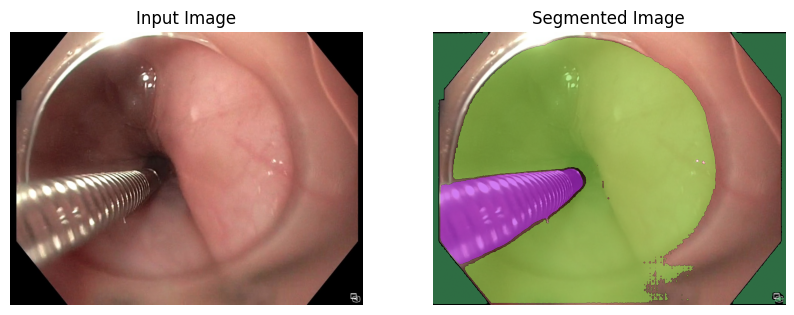
\includegraphics[width=0.4\textwidth]{Images/annoted.png}
    \caption{Annotated image \\ \textit{Background: Green, Muscle layer: Yellow, Electrode: Purple. There is no Mucosal layer in this image.}}
    \label{fig:annotated}
\end{figure}

\subsection{Architecture}

% writing the architecture of the model
A DeepLabv3 model with Resnet-101 backbone and FCN auxilary classifier is trained with data. 

\subsubsection{DeepLabv3}

DeepLabv3 is a semantic segmentation model that uses Atrous convolution to capture multi-scale context by using different dilation rates. It uses a ResNet-101 backbone with atrous convolution. The model uses atrous spatial pyramid pooling (ASPP) to capture multi-scale context by using different dilation rates. The model also uses a fully connected conditional random field (CRF) to refine the segmentation results. 
It take N feature maps as input from the ResNet-101 backbone and outputs N*4*H*W tensor, where N is the batch size, 4 is the number of classes, H is the height, and W is the width of the image.The model outputs a probability distribution over the classes for each pixel in the input image.  
\begin{figure}[ht]
    \centering
    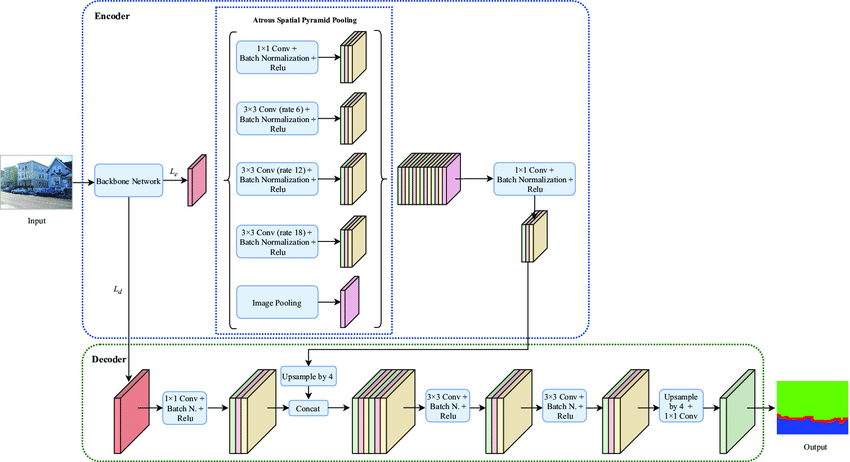
\includegraphics[width=0.6\textwidth]{Images/deeplabv3.png}
    \caption{DeepLabv3 architecture~\cite{deeplabv3-image}}
    \label{fig:deeplabv3}
\end{figure}

\begin{figure}[ht]
    \centering
    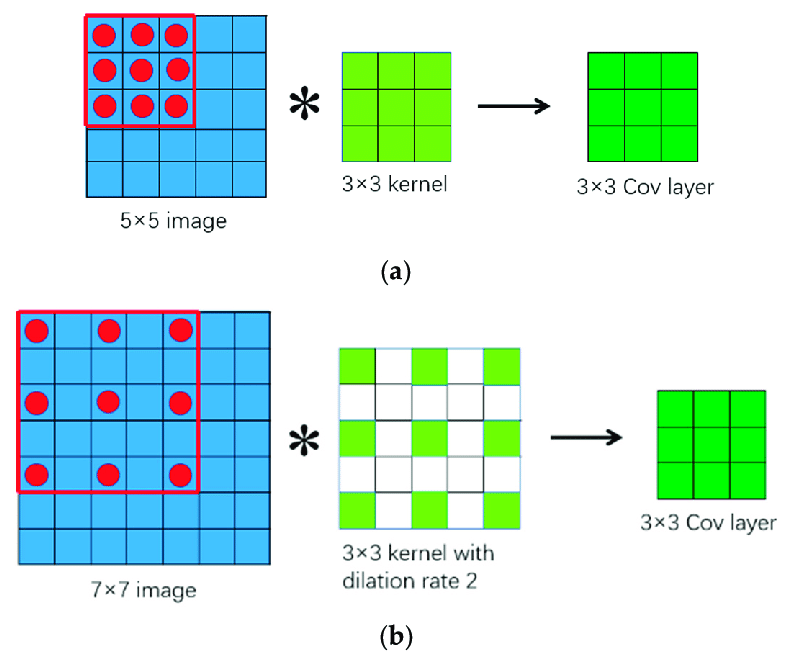
\includegraphics[width=0.5\textwidth]{Images/atrous-convolution.png}
    \caption{Atrous Spatial Pyramid Pooling (ASPP) in DeepLabv3\\ (a) Conv 3x3, rate=1 (b) Conv 3x3, rate=2 \\
    \cite{atrous-convolution-image}}
    \label{fig:atrous-convolution}
\end{figure}


\subsubsection{MobileNetV3-Large Backbone}

MobileNetV3-Large is a convolutional neural network designed for feature extraction. MobileNetV3-Large architecture uses 16 initial filters in the first convolution layer and then reduces the number of filters in the later layers by a factor of 2. It has typically 60 layers. Its building block involves an Inverted Residual Block, which includes a depth-wise convolution, a squeeze-and-excitation module, and a point-wise convolution. It takes normalized RGB im-
ages as input and outputs feature maps that are used by the
DeepLabv3 and the auxilary classifier. Input to the layer is
a 4-dimensional tensor with normalized RGB channels, and
the output is N*32*32, where N is the batch size. It involves downsampling layers.

\begin{figure}[ht]
    \centering
    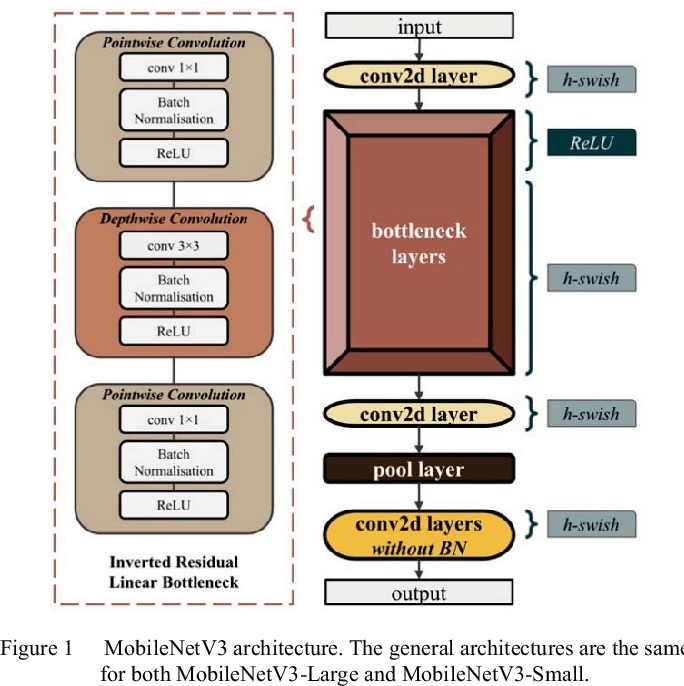
\includegraphics[width=0.5\textwidth]{Images/mobilenet-1.png}
    \caption{\cite{mobilenet-1}}
    \label{fig:mobilenet-1}
\end{figure}

\begin{figure}[ht]
    \centering
    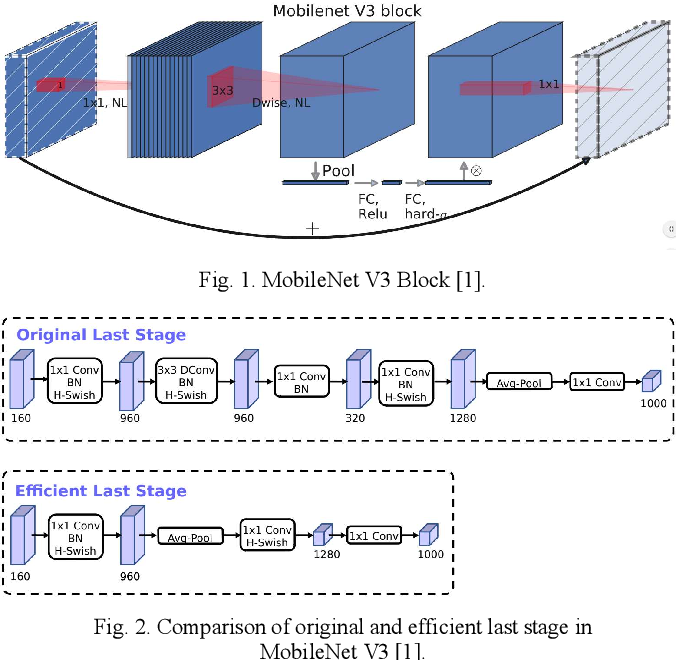
\includegraphics[width=0.5\textwidth]{Images/mobilenet-2.png}
    \caption{\cite{mobilenet-2}}
    \label{fig:mobilenet-2}
\end{figure}

\subsection{Training and Evaluation Setup}
While training on data, the input is a 4-dimensional tensor with normalized RGB channels, and the labels are 2D tensors with integer values representing the class labels for each pixel. The output from the PyTorch model is a 4-dimensional tensor with the shape (N, 4, H, W), where N is the batch size, 4 is the number of classes, H is the height, and W is the width of the output. The output is a probability distribution over the classes for each pixel in the input image. \\
The model is trained with the cross-entropy loss function. We use the Adam optimizer with learning rate scheduling with a step size of 1 epoch and a gamma of 0.8 (Initial Lerning rate = 0.001). Model is trained for 40 epochs with a batch size of 8. The model is trained on 70 images. The model is evaluated on 14 images. The evaluation metrics used are precision, mean intersection over union (mIoU), and pixel accuracy. 

 

\section{Architecture}

% writing the architecture of the model
A DeepLabv3 model with Resnet-101 backbone and FCN auxilary classifier is trained with data. 

\subsection{DeepLabv3}

DeepLabv3 is a semantic segmentation model that uses Atrous convolution to capture multi-scale context by using different dilation rates. It uses a ResNet-101 backbone with atrous convolution. The model uses atrous spatial pyramid pooling (ASPP) to capture multi-scale context by using different dilation rates. The model also uses a fully connected conditional random field (CRF) to refine the segmentation results. 
It take N feature maps as input from the ResNet-101 backbone and outputs N*4*H*W tensor, where N is the batch size, 4 is the number of classes, H is the height, and W is the width of the image.The model outputs a probability distribution over the classes for each pixel in the input image.  
\begin{figure}[h]
    \centering
    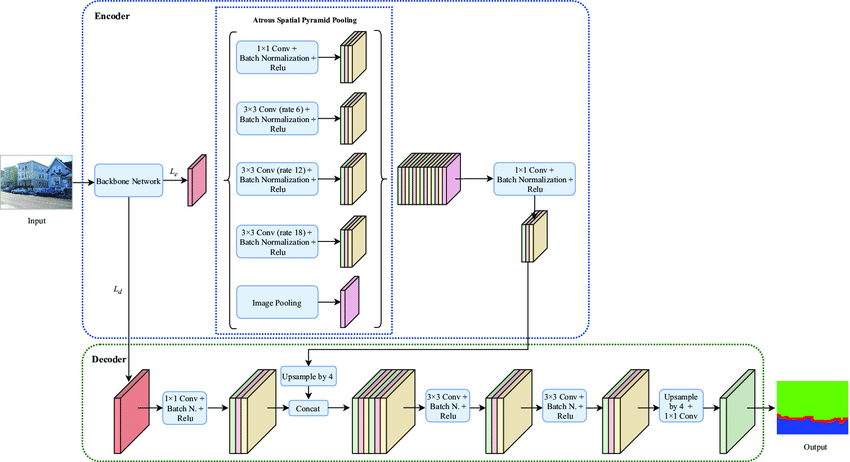
\includegraphics[width=0.6\textwidth]{Images/deeplabv3.png}
    \caption{DeepLabv3 architecture~\cite{deeplabv3-image}}
    \label{fig:deeplabv3}
\end{figure}

\begin{figure}[h]
    \centering
    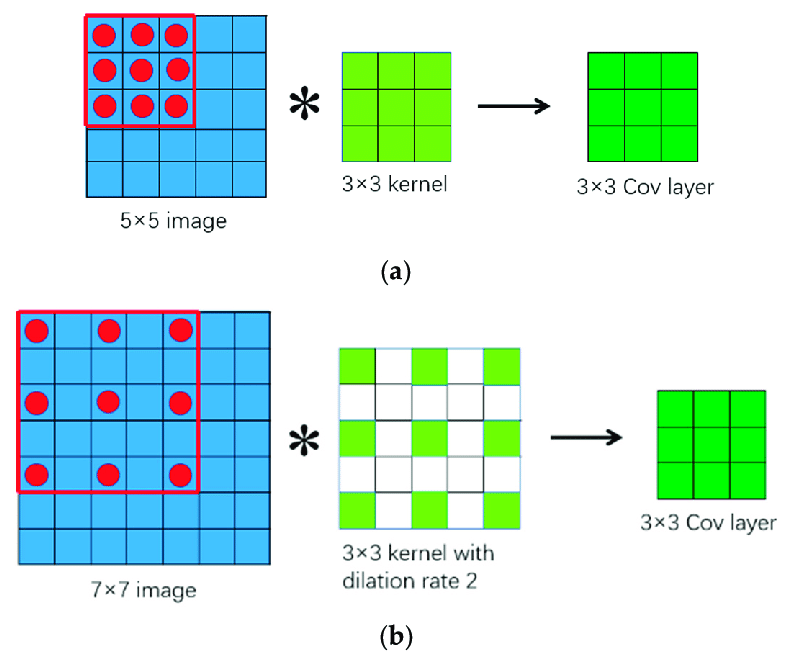
\includegraphics[width=0.5\textwidth]{Images/atrous-convolution.png}
    \caption{Atrous Spatial Pyramid Pooling (ASPP) in DeepLabv3\\ (a) Conv 3x3, rate=1 (b) Conv 3x3, rate=2 \\
    \cite{atrous-convolution-image}}
    \label{fig:atrous-convolution}
\end{figure}


\subsection{ResNet-101 Backbone}

Resnet-101 is convolutional neural network with 101 layers deep. It has residual blocks that allow the network to learn the identity function, which helps in training deeper networks. The residual blocks have skip connections that bypass one or more layers. It takes normalized RGB images as input and outputs feature maps that are used by the DeepLabv3 and the auxilary classifier. 
Input to the layer is a 4-dimensional tensor with normalized RGB channels, and the output is N*2048, where N is the batch size.  
Here, N = 1, as we are training the model with a single image at a time (small dataset).

\textbf{DeepLabv3 with a ResNet-101 backbone has approximately 53.5 million parameters.}

\begin{figure}[h]
    \centering
    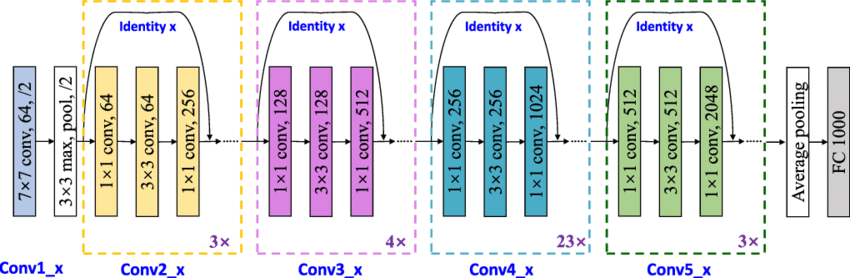
\includegraphics[width=0.5\textwidth]{Images/resnet.png}
    \caption{Residual blocks in ResNet-101 \cite{resnet-image}}
    \label{fig:resnet}
\end{figure}


\subsection{Auxilary Classifier}

The auxilary classifier is a fully connected layer that takes the feature maps from the ResNet-101 backbone and outputs a 4-dimensional tensor with the shape (N, 4, H, W), where N is the batch size, 4 is the number of classes, H is the height, and W is the width of the image. The auxilary classifier is used to improve the training of the model by providing additional supervision to the model. The output from the auxilary classifier is combined with the output from the DeepLabv3 model to improve the segmentation results.

\begin{lstlisting}
(aux_classifier):FCNHead(
(0):Conv2d(1024,256,kernel_size=(3,3),
    stride=(1, 1),padding=(1,1),bias=False)
(1):BatchNorm2d(256,eps=1e-05 momentum=0.1,
    affine=True)
(2):ReLU()
(3):Dropout(p=0.1,inplace=False)
(4):Conv2d(256,21,kernel_size=(1,1),
    stride=(1,1))
)
\end{lstlisting}{Architecture of the auxilary classifier in the model}

\subsection{Training Setup}
While training on data, the input is a 4-dimensional tensor with normalized RGB channels, and the labels are 2D tensors with integer values representing the class labels for each pixel. The output from the PyTorch model is a 4-dimensional tensor with the shape (N, 4, H, W), where N is the batch size, 4 is the number of classes, H is the height, and W is the width of the output. The output is a probability distribution over the classes for each pixel in the input image.
\\ The model is trained with the cross-entropy loss function, which is minimized using the Adam optimizer. The model is trained for 100 epochs. The learning rate is set to 0.01. The training takes approximately 30 mins to complete. The model is evaluated 3 images. The evaluation metrics used are precision, mean intersection over union (mIoU) and pixel accuracy.

\section{Results}
\label{sec:results}

We tested our model using the following metrics: epoch loss, pixel accuracy, IoU score, and dice score.

\begin{table}[htbp]
    \centering
    \caption{Performance metrics}
    \label{tab:example}
    \begin{tabular}{|c|c|c|}
        \hline
        \textbf{} & \textbf{Background} & \textbf{Muscle layer} \\
        \hline
        \textbf{Pixel accuracy} & 0.1875 & 0 \\
        \textbf{IoU score} & 0.45 & 0 \\
        \textbf{Dice score} & 0.00285 & 0 \\
        \hline
    \end{tabular} \\
    \begin{tabular}{|c|c|c|}
        \hline
        \textbf{} & \textbf{Mucosal layer} & \textbf{Electrode} \\
        \hline
        \textbf{Pixel accuracy} & 0 & 0 \\
        \textbf{IoU score} & 0 & 0 \\
        \textbf{Dice score} & 0 & 0 \\
        \hline
    \end{tabular} \\
\end{table}

\begin{figure}[!]
    \centering
    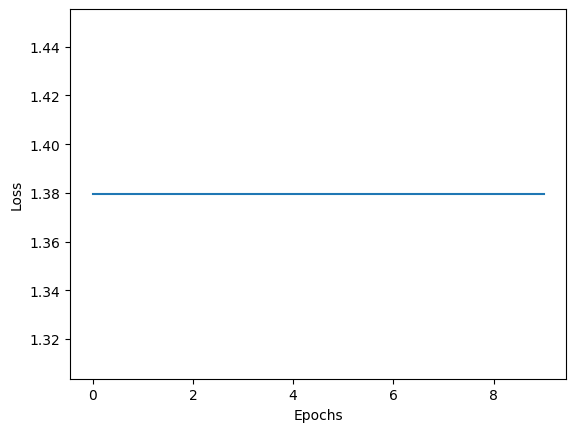
\includegraphics[width=0.4\textwidth]{Plots/loss}
    \caption{Epoch loss}
    \label{fig:loss}
\end{figure}

\begin{figure}[htp!]
    \centering
    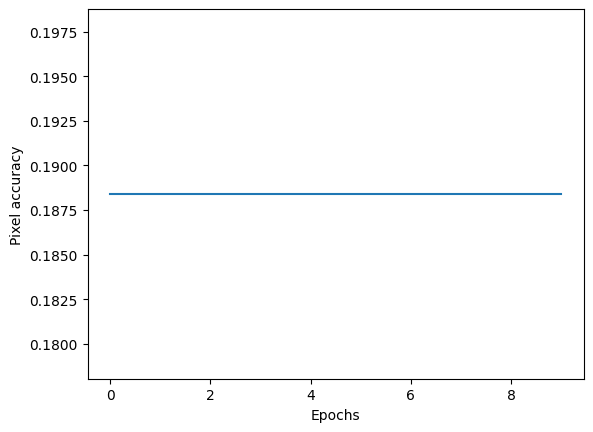
\includegraphics[width=0.4\textwidth]{Plots/accuracy}
    \caption{Pixel accuracy}
    \label{fig:accuracy}
\end{figure}

\begin{figure}[htp!]
    \centering
    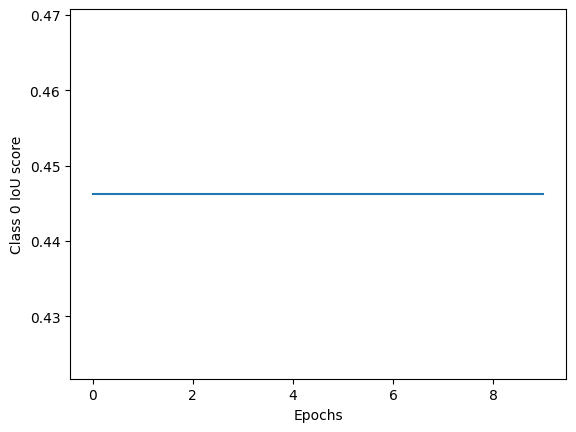
\includegraphics[width=0.4\textwidth]{Plots/iou}
    \caption{IoU score}
    \label{fig:iou}
\end{figure}

\begin{figure}[!]
    \centering
    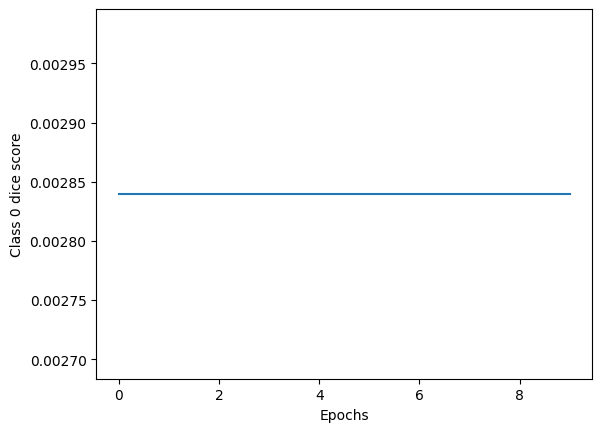
\includegraphics[width=0.4\textwidth]{Plots/dice}
    \caption{Dice score}
    \label{fig:dice}
\end{figure}

\section{References}

\begin{thebibliography}{00}
\bibitem{deeplabv3-image} https://www.researchgate.net/profile/Mma-Hashem/publication/352562164/figure/fig2/AS:1037138292396032@1624284446240/DeepLabv3-architecture.png

\bibitem{atrous-convolution-image} https://www.researchgate.net/publication/352562164/figure/fig1/AS:1037138292396032@1624284446239Illustrations-of-a-convolution-and-b-atrous-convolution.png

\bibitem{mobilenet-1} https://d3i71xaburhd42.cloudfront.net/7e0884e27643c212f32e9ab5dacfb552922eda07/2-Figure1-1.png

\bibitem{mobilenet-2} https://d3i71xaburhd42.cloudfront.net/915f986f1edce79cdde3c6ab7d335a7f14db4d2c/2-Figure1-1.png

\bibitem{sam-model} https://segment-anything.com/
\end{thebibliography}

{
    \small
    \nocite{*}
    \bibliographystyle{ieeenat_fullname}
    % \bibliography{main}
}

% WARNING: do not forget to delete the supplementary pages from your submission 
% \clearpage
\setcounter{page}{1}
\maketitlesupplementary


\section{Rationale}
\label{sec:rationale}
% 
Having the supplementary compiled together with the main paper means that:
% 
\begin{itemize}
\item The supplementary can back-reference sections of the main paper, for example, we can refer to \cref{sec:intro};
\item The main paper can forward reference sub-sections within the supplementary explicitly (e.g. referring to a particular experiment); 
\item When submitted to arXiv, the supplementary will already included at the end of the paper.
\end{itemize}
% 
To split the supplementary pages from the main paper, you can use \href{https://support.apple.com/en-ca/guide/preview/prvw11793/mac#:~:text=Delete%20a%20page%20from%20a,or%20choose%20Edit%20%3E%20Delete).}{Preview (on macOS)}, \href{https://www.adobe.com/acrobat/how-to/delete-pages-from-pdf.html#:~:text=Choose%20%E2%80%9CTools%E2%80%9D%20%3E%20%E2%80%9COrganize,or%20pages%20from%20the%20file.}{Adobe Acrobat} (on all OSs), as well as \href{https://superuser.com/questions/517986/is-it-possible-to-delete-some-pages-of-a-pdf-document}{command line tools}.

\end{document}
